\documentclass{article}

\usepackage[utf8]{inputenc}
\usepackage[T1]{fontenc}      
\usepackage[francais]{babel}
\usepackage{graphicx}
\usepackage{circuitikz}
\usepackage[squaren, Gray]{SIunits}
\usepackage{sistyle}
\usepackage[autolanguage]{numprint}
\usepackage{pgfplots}
\pgfplotsset{compat=1.9}
\usepackage{amsmath,amssymb,array}
\usepackage[top=2.5cm,bottom=2.5cm,right=2.5cm,left=2.5cm]{geometry}
\usepackage{url} 
\usepackage{tabularx}
\DeclareMathOperator{\dist}{d}
\newenvironment{abstract-fr}
{
	\begin{center}
		\textbf{Résumé} \\[0.5cm]
	\end{center}
}
{}

\newenvironment{abstract-en}
{
	\begin{center}
		\textbf{Summary} \\[0.5cm]
	\end{center}
}
{}
% New command pour la modélisation mécanique, tri à effectuer
\newcommand\fv[1]{{\bf #1}} % free vector
\newcommand\fvd[1]{\dot{\bf #1}} % free vector derivated
\newcommand\fvdd[1]{\ddot{\bf #1}} % free vector derivated
\newcommand\fvr[1]{\mathring{\bf #1}} % free vector relatively derivated
\newcommand\fvrr[1]{\overset{\circ\circ}{\bf #1}} % free vector relatively derivated
\newcommand\uv[1]{{\bf\hat{ #1}}} % unit vector
\newcommand\ui{{\bf\hat{I}}} % unit vector I
\newcommand\uj{{\bf\hat{J}}} % unit vector J
\newcommand\uk{{\bf\hat{K}}} % unit vector K
\newcommand\wrt[2]{\ensuremath{\tensor*[_{ #1}]{ #2}{}}} % With Respect To
\newcommand\wtr[3]{\ensuremath{\tensor*[_{ #1}]{ #2}{^{ #3}}}} % With Two Respect
\newcommand\omegaf{{\bm \omega}}
\newcommand\omegafr{\mathring{\bm \omega}}
\newcommand\omegafd{\dot{\bm \omega}}
\newcommand\omegaft{\tilde{\bm \omega}}
\newcommand\omegaftr{\mathring{\tilde{\bm \omega}}}
\newcommand\omegat{\tilde{\omega}}
\newcommand\omegatd{\tilde{\dot{\omega}}}
\newcommand\ine{{\bf I}}
\newcommand\st{{\bf L}}
\newcommand\pst{{\bf M}}
\newcommand\lm{{\bf N}}
\newcommand\am{{\bf H}}
\newcommand\amd{\dot{\am}}
\newcommand\fo{{\bf F}}
\newcommand\po{\mathcal{P}}
\newcommand\xg{\ensuremath{\fv{R}}}
\newcommand\xgd{\ensuremath{\fvd{R}}}
\newcommand\xgdd{\ensuremath{\fvdd{R}}}
\newcommand\dvec[1]{\dot{\vec{ #1}}}
\newcommand\ddvec[1]{\ddot{\vec{ #1}}}
\newcommand\qp{\dot{q}}
\newcommand\dqp{\Delta \dot{q}}
\usepackage{url} 
\usepackage{hyperref}
\hypersetup{
    colorlinks,
    citecolor=black,
    filecolor=black,
    linkcolor=black,
    urlcolor=black
}

\begin{document}

\section{La distorsion harmonique}

La distorsion est un critère de qualité en ce qui concerne les haut-parleurs.
Dans le soucis de construire un dispositif de qualité, nous avons décidé de 
nous informer sur la distorsion harmonique, un concept que nous ne connaissions
que de nom.
Ce document est structuré comme suit: nous parlerons tout d'abord de la notion  de distorsion 
en général pour ensuite aborder la notion  de distorsion 
harmonique, et finalement décrire ses causes, ses effets,
et les moyens de diminution.

\subsection{Définition}
Commençons tout d'abord par comprendre la notion de distorsion du son: par définition, c'est
une transformation du signal audio par rapport à celui de sortie. Une distorsion n'est généralement pas vraiment souhaitée, étant donné
que le signal en est déformé. Cependant, certains audiophiles en tirent avantage, vu que que quelques
transformations peuvent mener à un son plus agréable.

\paragraph{La distorsion harnomique}
La distorsion harmonique joue sur la superposition de différentes fréquences:
la fréquence fondamentale et ses harmoniques. Un haut-parleur parfait émettrait seulement la fréquence fondamentale, sans les harmoniques, qui sont donc des "parasites".
On parle d'harmonique pour désigner les multiples entiers de la fréquence fondamentale.
Par exemple, la seconde harmonique d'une fréquence de 50 Hz vaut 100Hz, la troisième 150Hz, etc. La figure 
ci-dessous illustre adéquatement cette notion.
Les harmoniques paires sont les moins incommodantes, étant donné qu'elles représentent la même note, mais à quelques octaves de différence.
Les harmoniques impaires, elles, sont plus gênantes étant donné que la note est différente.

\begin{figure}[ht!]
\centering
\scalebox{0.4}{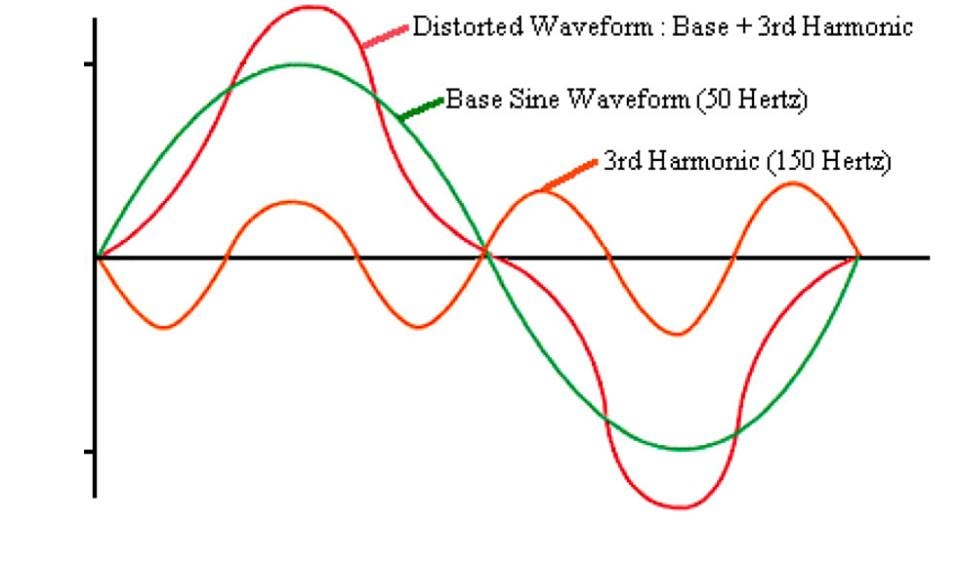
\includegraphics[scale=0.6]{distorsion.jpg}}
\caption{Superposition d'une fréquence fondamentale et de ses premières hamoniques.}
\label{Superposition d'une fréquence fondamentale et de ses premières hamoniques.}
\end{figure}

\subsection{Causes}
À cause de la distorsion harmonique, le signal que nous faisons circuler dans notre haut-parleur n'est pas
une sinusoïdale parfaite mais plutôt une série de Fourier, c'est-à-dire une somme de sinusoïdes de 
fréquence et d'amplitude différentes. C'est l'appareil en lui-même qui crée la distorsion, étant donné 
qu'il ne reproduit généralement pas parfaitement le signal d'entrée. 
Les charges non-linéaires sont les principales causes de distorsion harmonique. Celles-ci causent 
l'apparition des courants harmoniques qui sont eux-mêmes responsables de la distorsion harmonique.

\subsection{Conséquences}
La distorsion harmonique a plusieurs conséquences néfastes.
La plus importante de toutes vient du fait que les harmoniques impaires génèrent un son dur, et peu agréable. De plus, la distorsion cause un accroissement 
du courant dans un système. Il va en résulter une surchauffe des composantes électriques (conducteurs, 
capacités,...). À la longue, des disfonctionnements non souhaités peuvent provoquer un vieillissement 
précoce du circuit électrique. Il existe de nombreuses autres conséquences néfastes, mais n'oublions pas de préciser que certaines personnes recherchent tout de même ces distorsions pour produire un son plus agréable, au moyen d'harmoniques paires.

\subsection{Solutions}
Pour éviter toute distorsion, ou tout simplement pour émettre un son plus pur et exact, 
il existe différentes solutions. Nous parlerons seulement des filtres actifs 
mais il est intéressant de savoir que d'autre moyens existent.
Les filtres actifs permettent d'éliminer les harmoniques perturbatrices en injectant des courants
harmoniques de mêmes fréquences mais déphasés d'une demi-période. Cela cause des interférences
destructrices avec les harmoniques dont on souhaite se débarrasser. La résultante est une droite constante
nulle n'influençant pas notre signal.

% Just here to fix rapport_prejury.tex
\end{document}
